\section{模型五：六类潜在语音表型辅助分型}

\subsection{建模边界}

题目第五问涉及六类帕金森病症状，但数据集中没有静止性震颤、运动迟缓、肌肉僵直、疼痛、痴呆、睡眠障碍六类真实临床症状标签。因此，本文只在 Dataset 1 的 188 名 PD 受试者内部固定 \(k=6\) 进行无监督聚类，输出基于语音特征的六类潜在表型。六个 cluster 编号没有直接临床症状含义，仍需真实临床症状标签进一步验证。

\subsection{输入、方法与结果}

六类表型建模对 Top20、Top50 和 all acoustic 特征集进行候选方案比较，并做 \(k=2\) 到 \(k=8\) 的参考扫描。主方案为 \feature{top20_biomarkers} / \feature{pca_5} / AgglomerativeClustering。所有表示均先进行标准化，PCA 和聚类仅使用声学特征；二类聚类标签没有进入六类聚类输入。

\begin{table}[H]
\centering
\caption{六类潜在语音表型主方案指标}
\begin{tabularx}{\textwidth}{lY}
\toprule
项目 & 数值 \\
\midrule
主方案 & \feature{top20_biomarkers} / \feature{pca_5} / AgglomerativeClustering \\
PD 受试者数 & 188 \\
六簇人数 & 13、55、34、28、25、33 \\
最小簇比例 & 0.0691 \\
Silhouette & 0.1823 \\
Stability ARI mean & 0.4582 \\
二类与六类表型 NMI & 0.4089 \\
Collapsed majority ARI & 0.8128 \\
\bottomrule
\end{tabularx}
\end{table}

\begin{figure}[H]
\centering
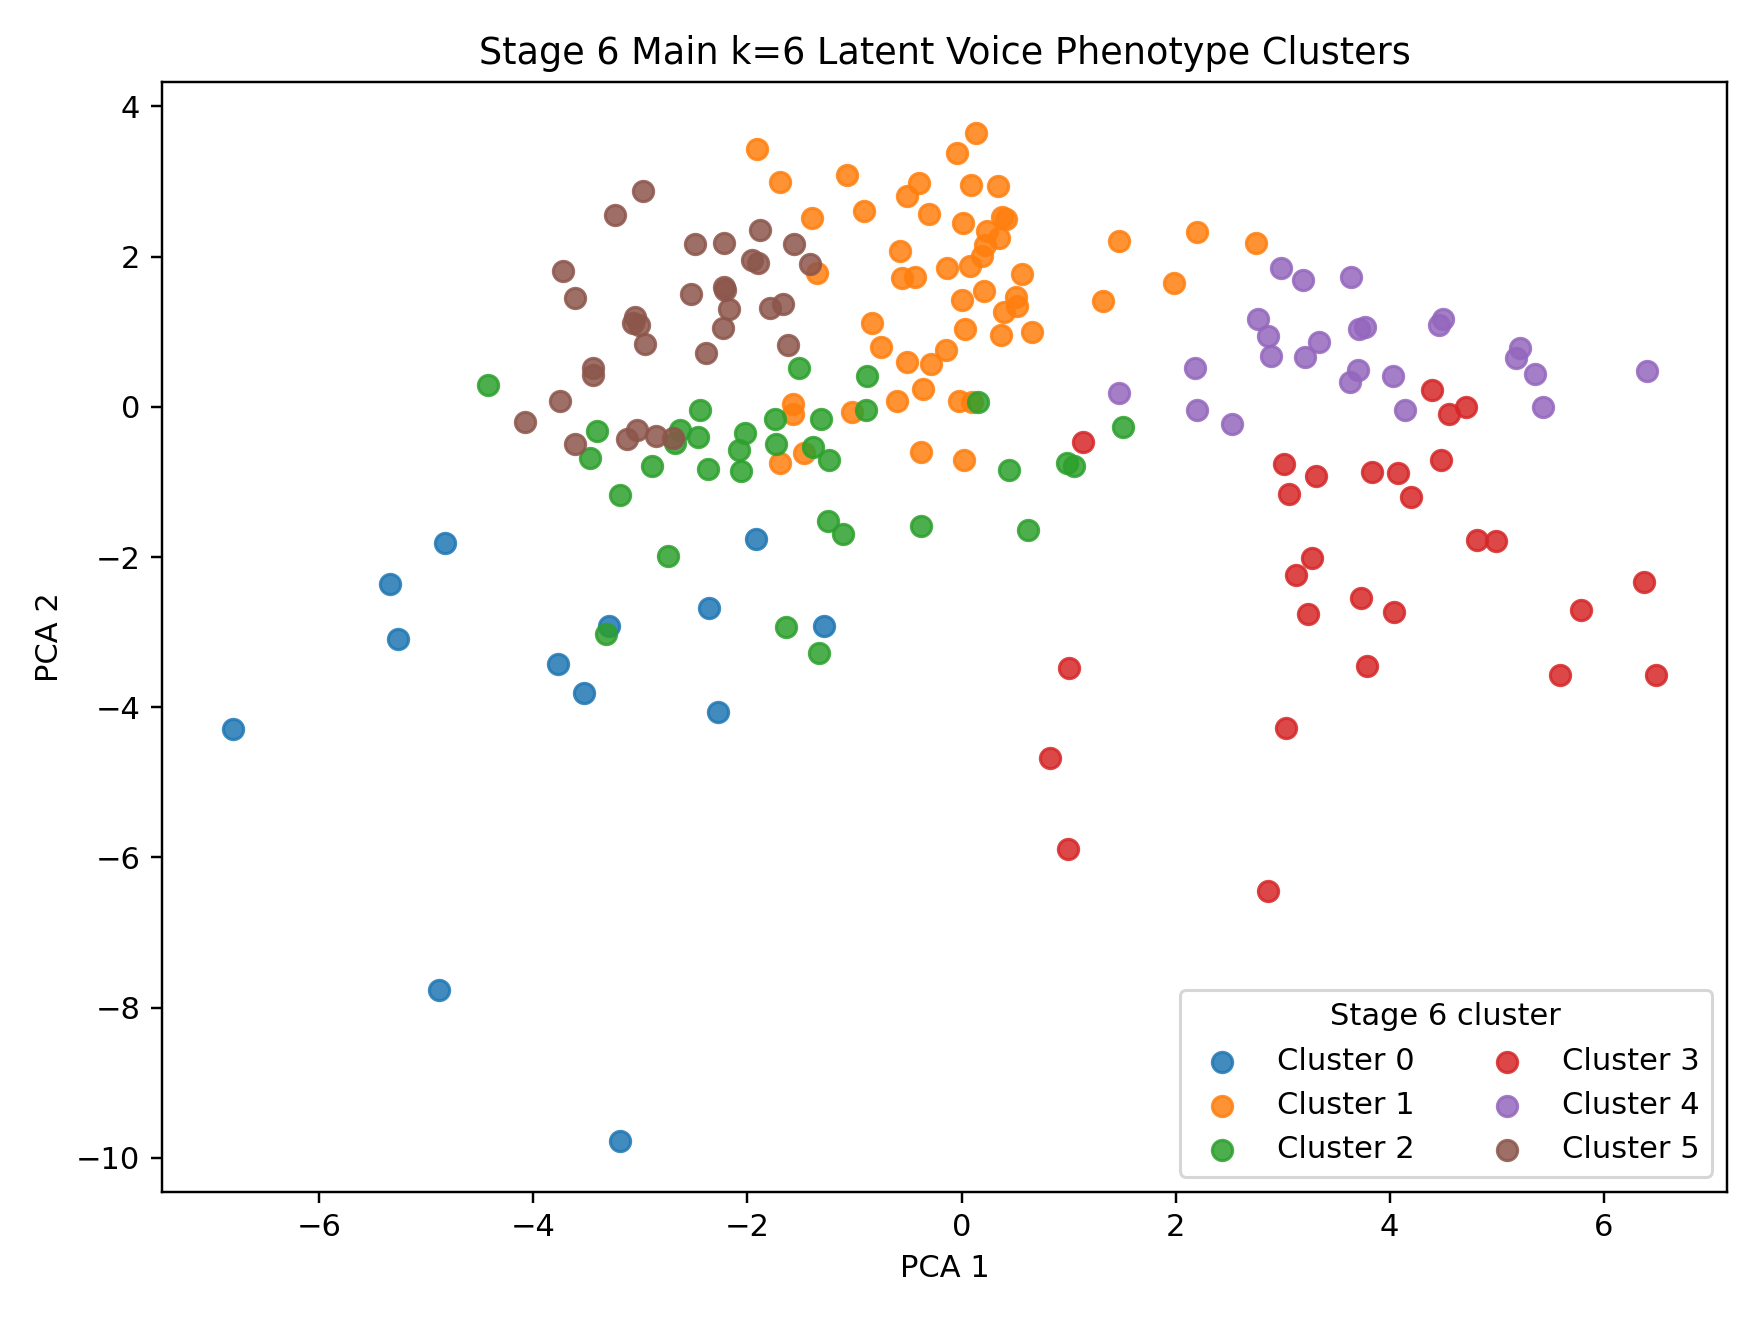
\includegraphics[width=0.84\textwidth]{figures/stage6_pca_k6_clusters_main.png}
\caption{Dataset 1 PD 受试者六类潜在语音表型 PCA 可视化}
\end{figure}

\begin{figure}[H]
\centering
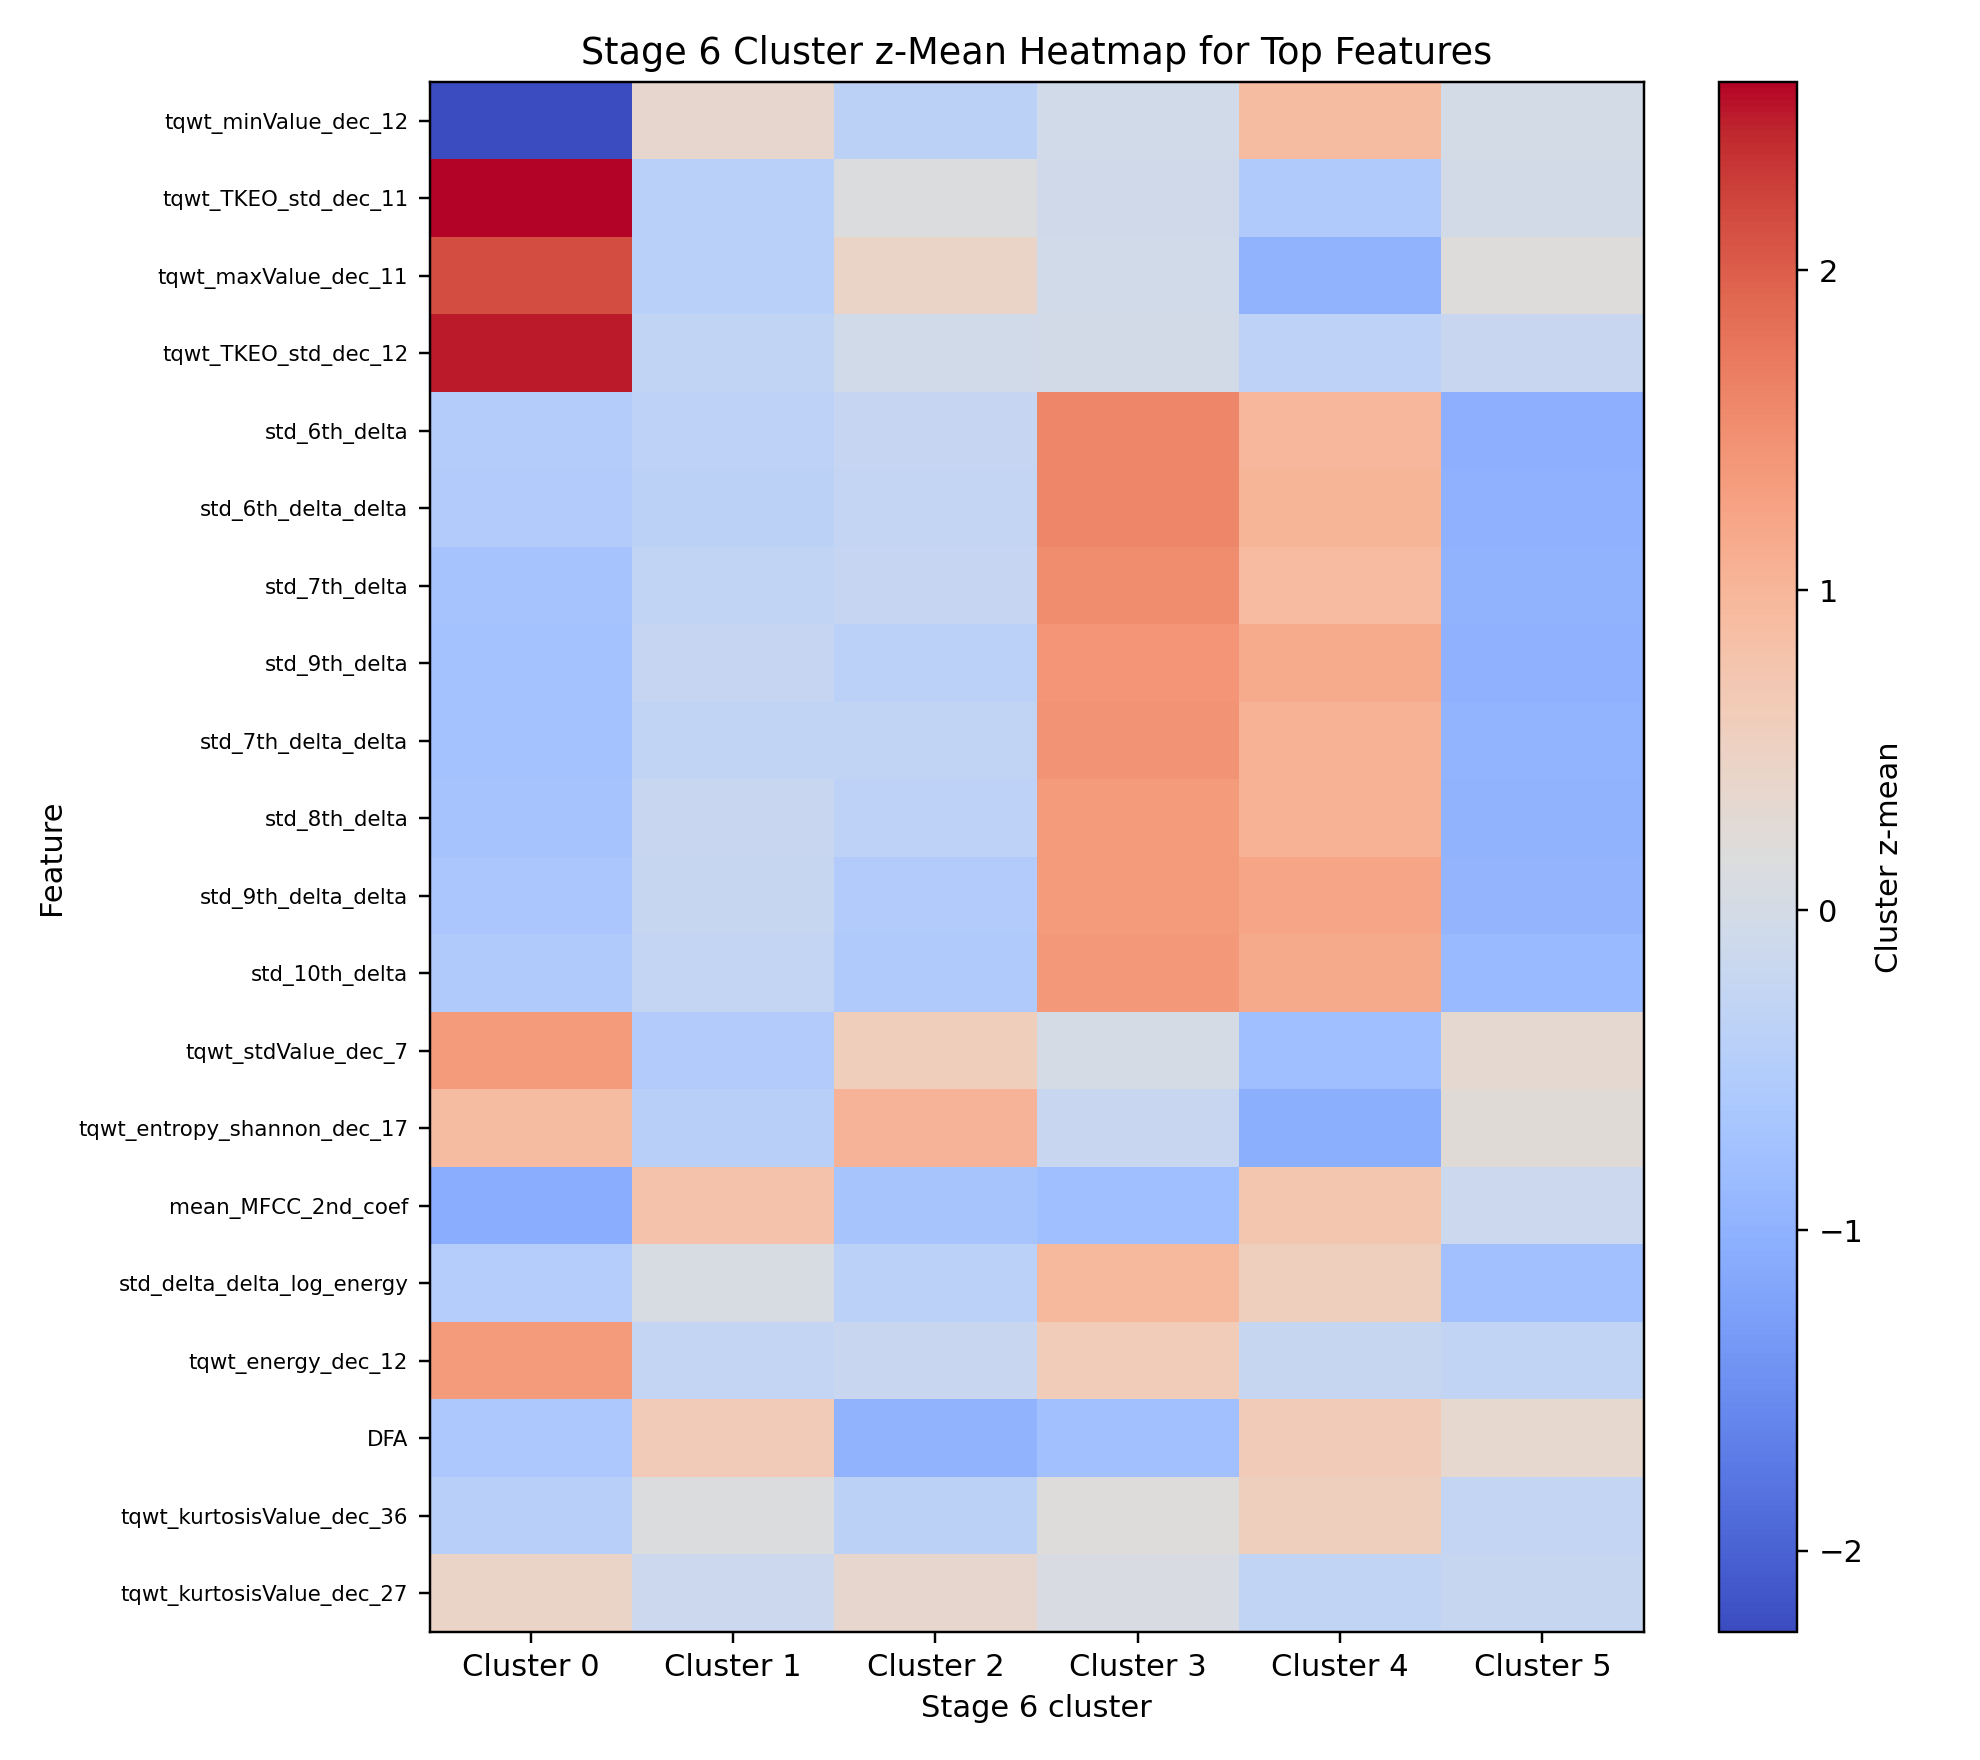
\includegraphics[width=0.9\textwidth]{figures/stage6_cluster_feature_heatmap.png}
\caption{六类潜在语音表型特征热图}
\end{figure}

\begin{figure}[H]
\centering
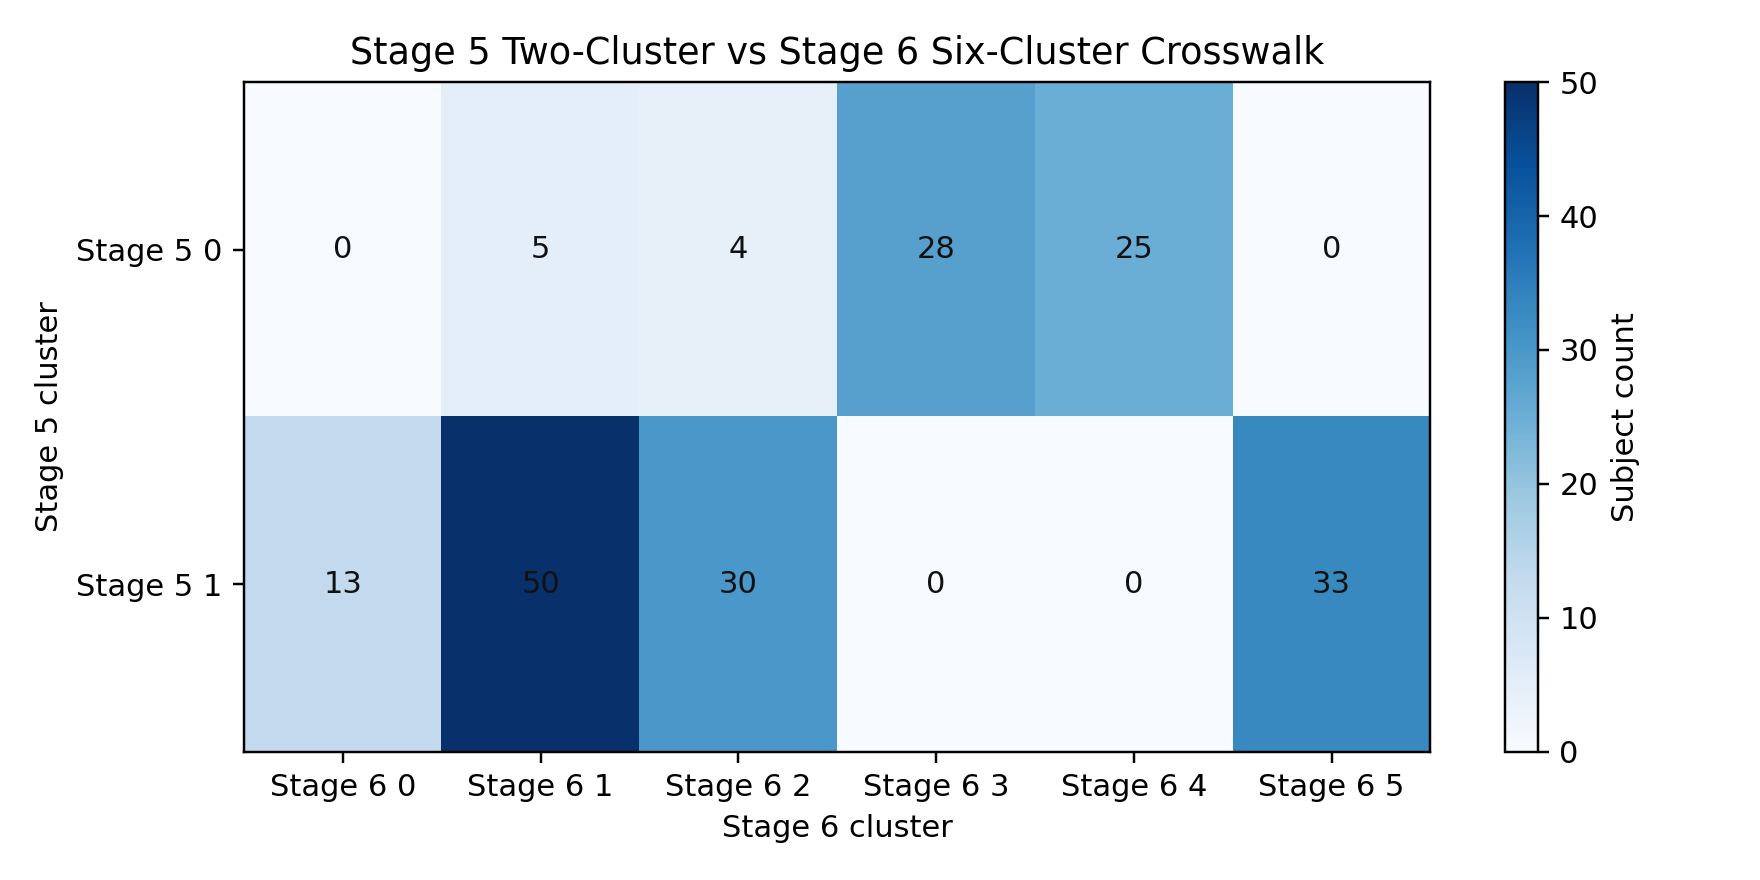
\includegraphics[width=0.76\textwidth]{figures/stage6_stage5_crosswalk_heatmap.png}
\caption{二类潜在表型与六类潜在表型交叉关系}
\end{figure}

\subsection{结果解释}

六类潜在语音表型主要由 Delta / Delta-delta 与 TQWT 特征区分。部分簇表现为动态谱波动特征较高，部分簇则表现为 TQWT 多尺度能量、熵或统计量差异。与二类方案相比，六类方案的 silhouette 下降到 0.1823，stability ARI mean 下降到 0.4582，说明固定 \(k=6\) 后聚类结构更细但稳定性和分离度较弱。

六类潜在表型与二类潜在表型存在一定嵌套关系，NMI 为 0.4089，按六簇多数映射回二簇后的 collapsed majority ARI 为 0.8128。该交叉关系只能说明六类潜在表型与二类潜在表型在声学空间中存在一定对应，不能解释为真实临床分层诊断。

六类聚类标签复现模型预测的是六类聚类标签，不是真实静止性震颤、运动迟缓、肌肉僵直、疼痛、痴呆或睡眠障碍标签。因此，其指标只表示复现无监督聚类划分的能力，不表示六类临床症状诊断能力。
